%%%%% Document Setup %%%%%%%%

\documentclass[12pt]{article}%{revtex4}    % Font size (12pt) and column number (one or two).

\usepackage{times}  % Times New Roman font type

\usepackage{natbib}

\usepackage{authblk}

\usepackage[a4paper, left=2.5cm, right=2.5cm,
 top=2.5cm, bottom=2.5cm]{geometry}         % Defines paper size and margin length

\renewcommand{\baselinestretch}{1.15}       % Defines the line spacing

\usepackage[font=small,
labelfont=bf]{caption}                      % Defines caption font size and caption title bolded

\usepackage{graphics,graphicx,epsfig,ulem}	% Makes sure all graphics works
\usepackage{amsmath}                        % Adds mathematical features for equations
\usepackage{float}
\usepackage{amssymb}
\usepackage{bm}
\usepackage{ltxgrid}

\usepackage{etoolbox}                       % Customise date to preferred format
\makeatletter
\patchcmd{\frontmatter@RRAP@format}{(}{}{}{}
\patchcmd{\frontmatter@RRAP@format}{)}{}{}{}
%\renewcommand\Dated@name{}
\makeatother

\def\thesection{\arabic{section}}

\def\bibsection{\section*{References}}      % Position reference section correctly

\def \apj {ApJ}                             % Define journal title shortcuts
\def \mnras {MNRAS}
\def \araa {Annual Review of Astronomy and Astrophysics}

\usepackage{hyperref}
\hypersetup{
    colorlinks=true,
    linkcolor=black,
    filecolor=magenta,      
    urlcolor=cyan,
    citecolor=black,
    pdftitle={Overleaf Example},
    pdfpagemode=FullScreen
    }

\urlstyle{same}

%%%%% Document %%%%%
\begin{document}                     
\onecolumngrid


\title{A Model for the Evolution of Quasars} 
\date{Submitted: \today{}}
\author{Joseph Carter}
\affil{\normalfont Level 4 Project, MPhys Physics with Astronomy\\ Supervisor: Professor T. Theuns\\ Department of Physics, Durham University}

\maketitle
%\thispagestyle{plain} % produces page number for front page

\begin{abstract}
 
\noindent In this project, we present a model for the formation and evolution of quasars based on the relationship between the evolution of quasars and their host galaxies, under the assumption that the formation rate of quasars is equal to the formation rate of galactic halos more massive than a critical mass $M_{H,crit}$ and that the lifetimes of quasars are related to the dynamical timescale of their host halos. Alternative models, in which quasar lifetimes are short, and where $M_{H,crit}$ varies with redshift, for either a constant critical halo virial velocity, $v_{H,crit}$, or for the halo mass above which star formation-driven outflows are no longer buoyant, are also investigated. Tests with our initial model using a constant $M_{H,crit}$ show that our model reproduces the redshift evolution of the quasar emissivity at 912\AA ($\epsilon_{912}$), calculated by \cite{Haardt_Madau}, well for $2\leq z\leq6$. By constraining the values of $M_{H,crit}$ and the quasar lifetime using minimum required black hole masses and by comparing the quasar number density to the predictions of \cite{Hopkins}, we conclude that the critical virial velocity and short quasar lifetime models cannot be used as they result in extremely low quasar number densities. The constrained values of the critical halo mass were found to be $M_{H,crit}=10^{11.73}M_\odot$ for the initial model, and $M_0=10^{12.08}M_\odot$ at $z=0$ for the outflow model. The required quasar lifetime was found to be $\sim10\times$ the dynamical timescale, leading to the conclusion that quasar lifetimes may not be related to the dynamical timescale, and are long enough that the loss rate of quasars does not become significant until after $z=2$. Using these parameters, both of these models maintained the good fit for the evolution of $\epsilon_{912}$ for $2\leq z\leq6$ found in the initial tests, but our models' estimates for the magnitude of the quasar UV emissivity were found to be $\sim1.5dex$ greater than the UV emissivity calculated by converting $\epsilon_{912}$. If the limitations of our model can be addressed in the future, it could be used to estimate both the evolution and magnitude of quasar emissivity for $2\leq z\leq6$.

\end{abstract}

\newpage

\tableofcontents
\newpage
\twocolumngrid
%\let\toc@pre\relax
%\let\toc@post\relax


\section{Introduction}

Almost all central galaxies (galaxies that are not satellites) are believed to contain a supermassive black hole (SMBH) at their centre.\\When a SMBH begins to rapidly increase in mass from accretion, the energy released from matter falling onto the black hole (BH) can exceed the luminosity of its host galaxy. These types of SMBH are known as active galactic nuclei (AGN). The most luminous AGN, with luminosities ranging between $~10^{11} - 10^{15}L_\odot$, are called quasars. In cosmology, quasars serve as important tools for studying the growth of black holes and the evolution of galaxies during the early stages of the Universe, and are believed to be the cause of the reionisation of the intergalactic medium (IGM). Since quasars are often very distant, and can be obscured by dust, measuring their properties, such as energy spectra and black hole masses, as well as global properties such as the number density and luminosity density (emissivity) of quasars, can often be difficult. Predictive models based on known properties of quasars are therefore useful tools, as they provide estimates for these difficult to measure properties.\par

The aim of this project is to develop a model for the formation and evolution of quasars using a model for galaxy formation which includes feedback from stars and accreting black holes. In this paper, we describe how the relation between the growth of SMBHs and the growth of their host galaxies can be used to determine the rate at which quasars are formed in the Universe, and how the formation rate of quasars can then be used to calculate quasar emissivity. Finally, we investigate how this model changes depending on factors such as quasar lifetimes, and the halo mass required for galaxies to host quasars.

\subsection{Overview}

The remainder of this section contains descriptions of the EAGLE simulations, which were used to produce most of the data used in this project, and the COLOSSUS python package for cosmology-related calculations. It is also shown that COLOSSUS can be used to produce halo mass functions which are a good fit for EAGLE data, as these are used in section 3 to estimate the formation rate of quasars. Section 2 discusses the motivation for this model. It is shown that many high mass galaxies have their star formation inhibited by AGN feedback, implying that there is a relationship between the mass of the galaxy and the presence or absence of an AGN. This relationship is discussed in further detail in section 3, and it is shown that the evolution of halo mass in EAGLE can be used to estimate the formation rate of quasars. The formation rate and number density of quasars are not easy quantities to measure, so in section 4, we explain how the emissivity of quasars can be calculated using the quasar formation rate produced by our model, and give an example with which this emissivity can be compared. In section 5, we introduce some alternative models with different requirements for a galaxy to host a quasar, and in section 6, we discuss how these models are affected when parameters such as quasar lifetimes are varied. Lastly, we discuss some limitations of our model and how they can be improved with further work in section 7.

\subsection{The EAGLE Simulations}

Unless stated otherwise, all of the plots in sections 1 to 3 were produced using data from the Virgo Consortium’s “Evolution and Assembly of GaLaxies and their Environments” simulation suite (EAGLE) (\cite{EAGLE}). This is a set of cosmological hydrodynamical simulations which use a modified version of the GADGET smoothed particle hydrodynamics code (\cite{GADGET}). All plots were produced using the Ref-L0100N1504 simulation. Full details of the parameters used in the simulations can be found in the EAGLE paper. In EAGLE, halos that exceed a certain mass are given a 'seed' SMBH with an initial mass of $10^5M_\odot$.

\subsection{COLOSSUS}

The plots in sections 4 to 6 were produced using COLOSSUS (\cite{COLOSSUS}). This is a Python package for calculations related to cosmology, the large-scale structure of matter in the Universe, and the properties of dark matter halos. In particular, it is used in this project to produce halo mass functions, as well as calculating the values of cosmological parameters, and converting between redshift and cosmic time. It is shown in section 1.4 that the mass functions produced by COLOSSUS are a good fit for mass functions produced using data from EAGLE.\par

The python code used to create the plots used in this paper can be found \href{https://github.com/xvh422/L4-Project/blob/main/J_Carter_Code.ipynb}{here}. Please note that this code is not well documented, and its readability is limited, but has been shared regardless for the purpose of reproducability.

\subsection{Comparing the Halo Mass Functions of EAGLE and COLOSSUS}

Halo mass functions for EAGLE galaxies at various redshifts are plotted alongside halo mass functions from COLOSSUS in Figure 1 for comparison. The large uncertainties on the lower values of the EAGLE mass functions are due to the small number of high mass galaxies present in the simulation. It can be seen from Figure 1 that COLOSSUS produces mass functions that are a good fit for the measured mass functions from EAGLE. Additionally, the mass functions from COLOSSUS do not suffer from the same lack of measurable high mass galaxies as EAGLE, which is the cause for the large error in the EAGLE mass functions at higher masses, as seen in Figure 1. COLOSSUS is also computationally simpler and faster than using queries to obtain data from EAGLE.\par

As a result of these advantages, the comoving number density of halos of a given mass, plotted as a function of redshift, is used in section 3 to compute the rate at which galaxies transition from the blue cloud to the red sequence, and hence the rate at which quasars are formed as a function of redshift.

\begin{figure}[H]
\centering
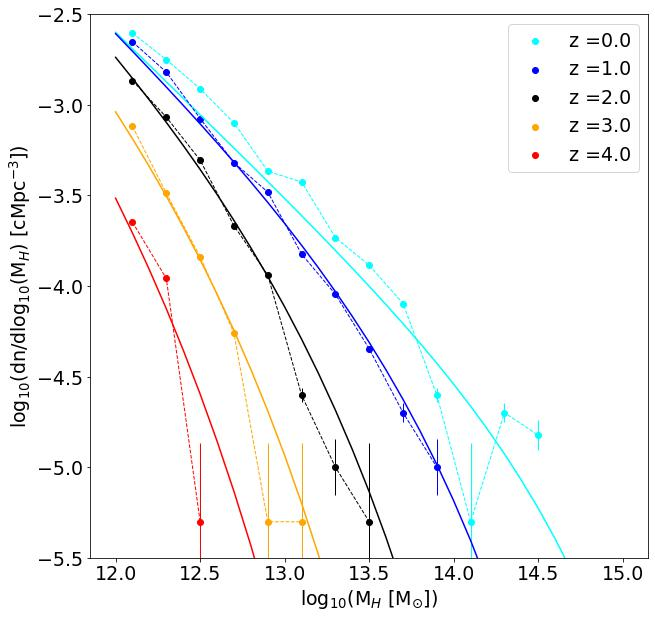
\includegraphics[width=\linewidth]{Mass_Function.jpeg}
\caption{Halo mass functions for galaxies of halo mass greater than $10^{12}M_\odot$ between $z=0$ and $z=4$. The dashed lines show mass functions from EAGLE, filled lines show mass functions from COLOSSUS, which have been converted to be in terms of $log_{10}(M_H)$ instead of their standard units of $ln(M_H)$ to match with units from EAGLE.}
\label{fig:1}
\end{figure}

\onecolumngrid


\begin{figure}[H]
\centering
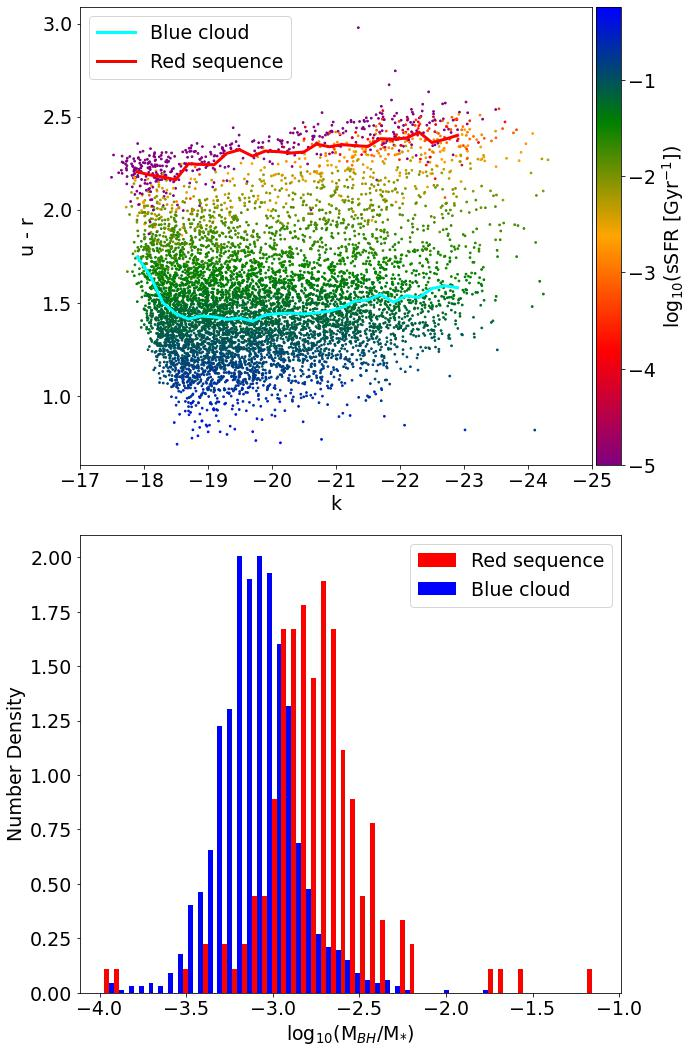
\includegraphics[width=14.5cm]{Plot_1.jpeg}
\caption{Top: u-r magnitude as a function of k-band magnitude for galaxies of stellar mass $\gtrsim10^9M_\odot$ at $z=0$. k-band magnitude is strongly correlated to stellar mass, so brighter galaxies can be taken to have higher stellar mass. Individual galaxies are plotted as points, coloured by sSFR, using the colourbar to the right. Bottom: histogram of $M_{BH}/M_*$ for galaxies of stellar mass between $10^{10} - 10^{10.5}M_\odot$, separated into blue cloud galaxies and red sequence galaxies.}
\label{fig:2}
\end{figure}
\twocolumngrid


\section{The Effect of AGN Feedb\-ack on Star Formation}

The top plot of Figure 2 shows the relationship between u-r magnitude, which shows how blue (low magnitude) or red (high magnitude) an object is, and k-band magnitude, which is strongly correlated to stellar mass, for galaxies of mass greater than $10^9M_\odot$. It can be seen that the galaxy population in EAGLE is divided into a highly star forming 'blue cloud' which contains the majority of galaxies with stellar mass below $10^{10}M_\odot$ and a 'red sequence' with a significantly lower specific star formation rate\\(sSFR), which contains a significant amount of the high-mass galaxies (many of the galaxies in Figure 2 actually have an sSFR of 0, but have been equated to the lowest non-zero sSFR so that they can be shown on a log plot). The difference in star formation rate between the blue cloud and the red sequence is believed to depend on the type of feedback present in the galaxy. Star formation in blue cloud galaxies is regulated by  stellar feedback, in which the energy injected into the interstellar medium by supernovae balances the energy lost due to cosmological \hspace{2.5mm} accretion \hspace{2.5mm} (\cite{Ikea}). However, for galaxies with dark matter halos more massive than a critical mass of $M_{H,crit}\sim10^{12}M_\odot$ outflows driven by supernovae will no longer be buoyant, leading to a buildup of gas in the central regions of the galaxy. This allows the central black hole to grow rapidly, quickly reaching sufficient mass to begin AGN feedback, in which energy released by the black hole heats the gas corona surrounding the galaxy, disrupting the inflow of cold gas and suppressing star formation.\\More evidence of this can be seen from the colour of the points in Figure 3, as this shows a decrease in sSFR for galaxies with high BH mass and halo mass. The lower histogram of Figure 2 shows the difference in the ratio between BH mass and stellar mass for galaxies in the blue cloud and the red sequence. The histogram peaks at a higher value for the red sequence than for the blue cloud, implying that red sequence galaxies, on average, have a more massive BH compared to the mass of the host galaxy than for blue cloud galaxies. This provides further evidence that AGN feedback is responsible for the low star formation in the red sequence, as AGN are typically more massive than inactive SMBH's due to their high accretion rates.\par

\vspace*{1cm}

Since the presence of an AGN is believed to be the cause of galaxies making the transition from the blue cloud to the red sequence, measuring the number of galaxies which exceed $M_{crit}$ and therefore transition to the red sequence at a given redshift will also provide a measurement of the number of quasars formed at that redshift. This provides the motivation for our model, and is discussed further in section 3.

\section{Relating Halo Mass to the Formation Rate of Quasars}
\subsection{The Black Hole Mass - Halo Mass Relation}

Figure 3 shows the black hole mass - halo mass relation for central galaxies of stellar mass $\geq10^9M_\odot$. There appears to be little to no correlation at low halo masses, and the gaps with no points are due to black holes growing suddenly via mergers instead of continuously via accretion. For halo masses above $~10^{11.5}M_\odot$, black hole mass and halo mass appear to be correlated. One problem when determining which

\onecolumngrid


\begin{figure}[H]
\centering
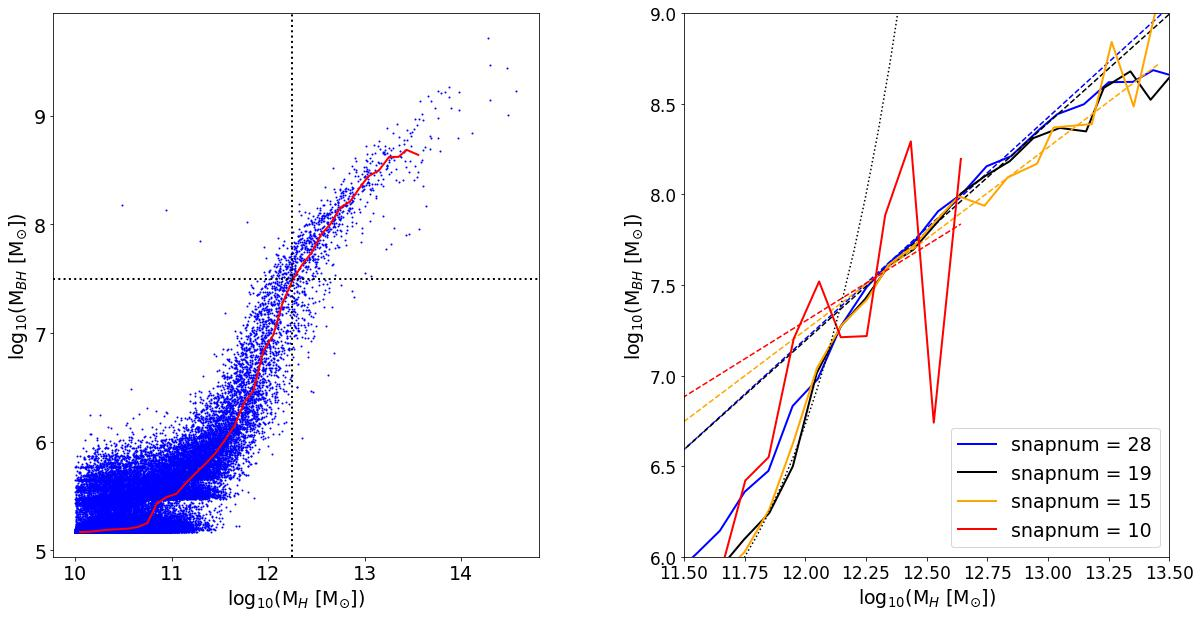
\includegraphics[width=17cm]{Plot_3.jpeg}
\caption{Left: Black hole mass - halo mass relation for central galaxies of stellar mass $\gtrsim10^9M_\odot$ at $z=0$, the blue line shows median black hole mass. Individual halos are plotted as points, coloured by sSFR, using the colourbar to the right. The dotted lines show BH mass (horizontal) and halo mass (vertical) at the beginning and end of the qso phase. Right: Median black hole mass as a function of halo mass for central galaxies at snapnums 28, 19, 15, and 10 (equivalent to z = 0, 1, 2, and 4 respectively). Dashed lines show power law fits, the dotted line shows an exponential fit.}
\label{fig:3}
\end{figure}
\twocolumngrid


\noindent black holes are accreting at close to the Eddington rate is that the instantaneous black hole accretion rates measured in EAGLE have a very large scatter, but it is known that halos increase in mass with cosmic time, so halos plotted on Figure 3 can be assumed to contain black holes that are growing according to the relation shown in Figure 3.

The right plot of Figure 3 shows that black hole mass follows an exponential fit for medium-mass halos, so halos that lie on the exponential curve (those between the vertical dotted lines) can be assumed to contain black holes that are growing exponentially, following the BH mass - halo mass relation, and halos that lie on the power law fit (those at higher masses than the exponential curve) can be assumed to contain black holes that are growing according to a power law. The exponential growth region seems promising for approximately Eddington limited black hole growth, but the black hole masses in this region are significantly lower than the measured masses of real quasars, which can have masses of $\sim10^9M_\odot$ (\cite{Marshall}). This could be a result of the approximation in EAGLE that all SMBHs start as seeds of a specific mass. However, it is shown in \cite{Quasar} that the seed mass of the SMBHs has little effect on their final mass. Additionally, although the instantaneous BH accretion rates in EAGLE have a large scatter, it can be seen from Figure 4 that the Eddington ratios (accretion rate divided by Eddington rate) of the highest mass black holes do not appear to differ much from the Eddington ratios of $10^{6.5-7.5}M_\odot$ black holes. Therefore, the most luminous AGN should be the more massive black holes on the power law fit.

\begin{figure}[H]
\centering
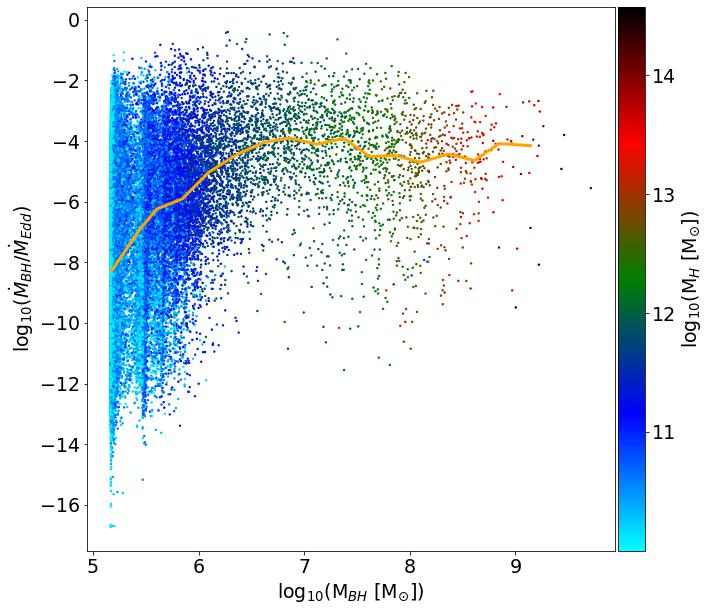
\includegraphics[width=\linewidth]{Plot_12.jpeg}
\caption{Instantaneous Eddington ratio - BH mass relation for halos more massive than $10^{10}M_\odot$. Individual halos are plotted as points, coloured by halo mass. The orange line shows median Eddington ratio, and appears to increase up to a BH mass of $\sim10^{6.5}M_\odot$, before its evolution stops.}
\label{fig:4}
\end{figure}

 \subsection{Calculating the Quasar Formation Rate}

 \begin{figure}[H]
\centering
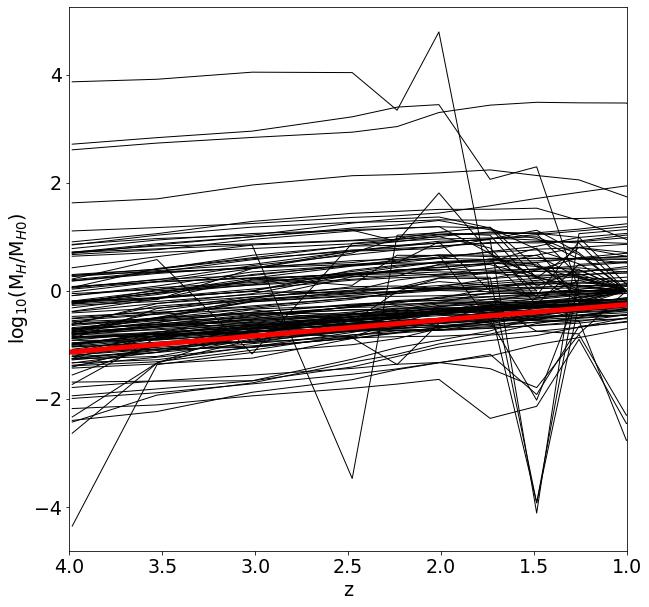
\includegraphics[width=\linewidth]{Plot_5.jpeg}
\caption{The black lines show $M_H/M_0$ as a function of redshift for central galaxies which cross the $10^{12}M_\odot$ halo mass threshold at z=2. The red line shows $M_H/M_0$ as described by Equation (3).}
\label{fig:5}
\end{figure}

The median black hole mass on the left plot of Figure 3 reaches a high enough BH mass for a luminous AGN at a halo mass of $\sim10^{12}M_\odot$. Our model assumes that the rate at which quas\-ars are formed is equal to the rate at which galaxies cross the $10^{12}M_\odot$ halo mass threshold: $\frac{dn}{dz}$, where n is the number of galaxies of halo mass greater than $10^{12}M_\odot$ per unit comoving volume. This can be calculated using (\cite{Correa}):

\begin{equation}
    \frac{dn}{dz}=\frac{dn}{dln(M_H)}\frac{dln(M_H)}{dz}
\end{equation}

\noindent where $dn/dln(M_H)$ is the comoving number density of halos with mass $M_H=10^{12}M_\odot$ at a given redshift, which can be calculated from halo mass functions produced using COLOSSUS, and the logarithmic growth rate is given by:

\begin{equation}
    \frac{dln(M_H)}{dz}=\frac{a}{(1+z)}-b
\end{equation}

\noindent This corresponds to the parametrisation described by \cite{Correa}, in which $M_H$ can be written as:

\begin{align}
    \frac{M_H}{M_0}&=m_H(z) \nonumber \\
    m_H(z)&\approx(1+z)^ae^{-bz}
\end{align}

\noindent where a and b are fitting parameters, and $M_0$ is the value of $M_H$ at $z=0$. \citeauthor{Correa} give values for a \& b, averaged over halo masses, as $\bar a \approx 0.24, \bar b \approx 0.75$, but to test their fit for the evolution of EAGLE galaxies crossing the $10^{12}M_\odot$ halo mass threshold, $M_H/M_0$ is plotted against z in Figure 5 for EAGLE galaxies and for $m_H(z)$. Figure 5 shows that Equation (3) fits the evolution of halo mass with redshift well for EAGLE galaxies crossing the $10^{12}M_\odot$ halo mass threshold (outliers in Figure 5 that are significantly more massive than they are at $z=0$ are believed to be caused by halos passing through one another and contributing to each others' measured masses, before moving away at $z\approx0$, leading to  sudden decreases

\onecolumngrid


\begin{figure}[H]
\centering
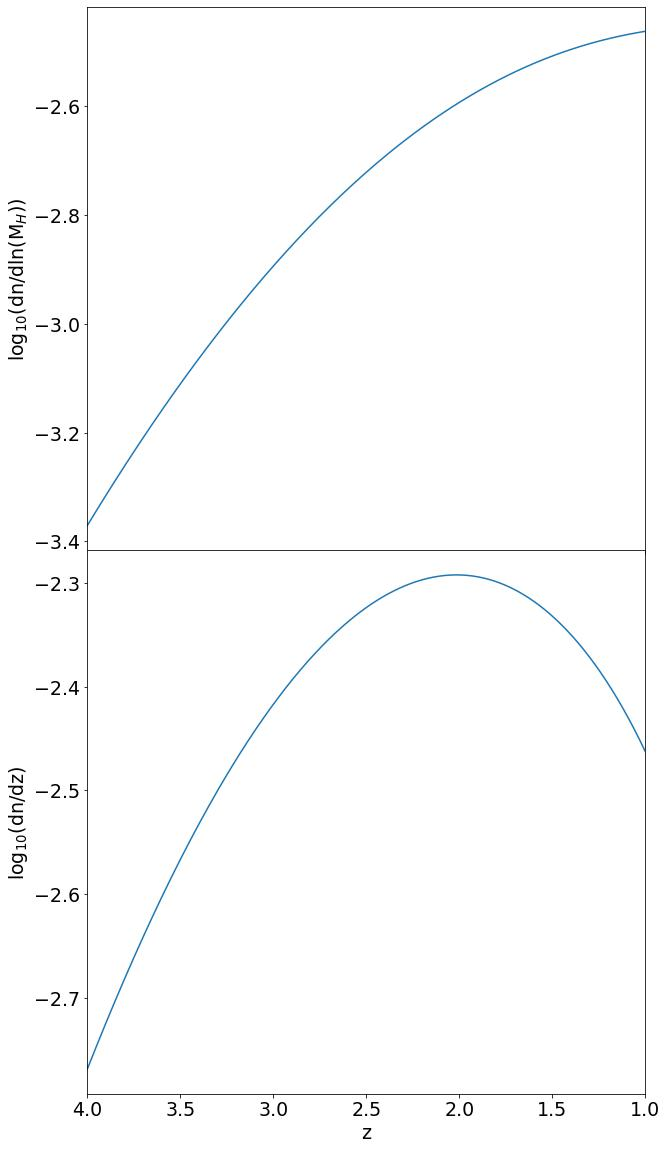
\includegraphics[width=12.5cm]{Plot_6.jpeg}
\caption{Top: Comoving number density of halos with mass $10^{12}M_\odot$ as a function of redshift, produced using COLOSSUS. Bottom: Formation rate of halos of mass greater than $10^{12}M_\odot$ as a function of redshift, calculated using Equation (2). This appears to peak at $z\approx1$.}
\label{fig:6}
\end{figure}
\newpage
\twocolumngrid


\noindent in the measured value of $M_H$). This means that the constant values of $\bar a$ and $\bar b$ can be substituted into Equation (2)

\begin{equation}
    \frac{dln(M_H)}{dz}=\frac{\bar a}{(1+z)}-\bar b
\end{equation}

\noindent meaning that $dln(M_H)/dz$ and $dn/dln(M_H)$ are now functions of z only.\par

The top plot of Figure 6 shows the comoving number density of halos with mass $10^{12}M_\odot$, $dn/dln(M_H)$, for reference, and in the bottom plot, $dln(M_H)/dz$ and $dn/dln(M_H)$ are multiplied as in Equation (1) to produce a plot of the formation rate of halos with mass greater than $10^{12}M_\odot$, and hence the formation rate of quasars, $dn/dz$, as a function of redshift. The formation rate peaks at $z\approx1$ before decreasing for $0\leq z\lesssim1$.

\section{Calculating Quasar Emissivity}

Our model now has a prediction for the formation rate of quasars, and the number density of quasars can be calculated from this, but these quantities are difficult to measure for the real Universe. A measurable quantity which can also be calculated from this model is the quasar emissivity in a particular region of the EM spectrum, such as UV.\par

To obtain an estimate for quasar emissivity, the number density of quasars must first be calculated from the formation rate, and this in turn requires an estimate of the lifetime of each quasar. This section discusses how the quasar lifetime can be estimated, and then shows how the quasar emissivity can be calculated from this, and finally compares the results of these methods with quasar emissivity calculated by \cite{Haardt_Madau}.

\subsection{Calculating Quasar Emissivity in our Model}

The lifetimes of quasars are not very well understood. One possibility is that, since the black hole’s growth is driven by accreting material that falls into the centre of the halo, the quasar’s lifetime could be proportional to the dynamical timescale of the host halo:

\begin{equation}
    \tau\propto t_{dyn}=\frac{1}{\sqrt{G\rho}}
\end{equation}

\noindent This is the minimum time taken for a uniform gas cloud with density $\rho$ to collapse, and so would be approximately equal to the time taken for all the gas present in the halo at the start of the quasar phase to fall to the centre and drive the black hole’s accretion. By substituting $\Bar{\rho}_{halo}=200\Bar{\rho_{crit}}=200\frac{3H^2}{8\pi G}$ and rearranging, we obtain:

\begin{equation}
    t_{dyn}=\left(\frac{300}{4\pi}\right)^{-\frac{1}{2}}t_H
\end{equation}

\noindent where $t_H$ is the Hubble time. This leads to a final expression for the quasar lifetime:

\begin{equation}
    \tau=k\left(\frac{300}{4\pi}\right)^{-\frac{1}{2}}t_H
\end{equation}

\noindent where k is a proportionality constant.\par

To calculate the number density of quasars, a "loss rate" is first produced by delaying the formation rate, $\frac{dn}{dt}=\frac{dn}{dz}\frac{dz}{dt}$, by the assumed quasar lifetime (see left plot of Figure 7). The quasar number density is then calculated by numerically integrating the formation rate with respect to time, then subtracting the numerical integral of the loss rate:

\begin{equation}
    n(t)=\int_{t_0}^t\frac{dn}{dt'}dt'-\int_{t_0+\tau(t=t_0)}^tl(t')dt'
\end{equation}

\noindent where $l(t)$ is the quasar loss rate and $\tau(t=t_0)$ is the assumed quasar lifetime at $t=t_0$. Ideally, $t_0$ would be zero, but this corresponds to $z=\infty$ and would be unsuitable for calculations using COLOSSUS, so $t_0$ is instead chosen to be a finite cosmic time reasonably close to zero. The comoving quasar number density calculated using this method can be seen in the right plot of Figure 7.\par

Another quantity required to calculate the quasar emissivity is the total amount of energy radiated by a quasar during its lifetime. This can be calculated using:

\begin{equation}
    E=\eta M_{BH,final}c^2
\end{equation}

\noindent where $\eta$ is the efficiency at which accreted mass is converted to radiation, assumed here to be 0.1, and $M_{BH,final}$ is the final mass reached by the quasar. Because of the difficulties associated with measuring the masses of quasars, the final black hole mass is simply estimated to be $10^{8.5}M_\odot$, but this final mass will be investigated further in section 6.\par

Now that expressions have been obtained for the quasar number density, lifetime, and the total energy released by each quasar, the comoving quasar emissivity can be calculated using:

\begin{equation}
    \varepsilon_{model}=n\frac{E}{\tau}
\end{equation}

\subsection{Quasar Emissivity at 912\AA}

In \cite{Haardt_Madau}, the function:

\begin{multline}
    \frac{\epsilon_{912}(z)}{(1+z)^3}=(10^{24.6}erg s^{-1}Mpc^{-3}Hz^{-1})\\
    \times(1+z)^{4.68}\frac{exp(-0.28z)}{exp(1.77z)+26.3}
\end{multline}

\noindent is used to calculate the comoving quasar emissivity at the frequency corresponding to a wavelength of 912\AA, this also corresponds to an energy of 1ryd - the ionisation energy of hydrogen. The evolution of emissivity with redshift can be directly compared between this formula and our model. This is shown in Figure 8, where it can be seen that the evolution of the emissivity produced using our model appears to be a good fit for the evolution of the emissivity at 912\AA \: calculated by \cite{Haardt_Madau} between redshifts $2\lesssim z\lesssim6$. Additionally, the emissivities peak at the same redshift. The only major deviation from the prediction of \citeauthor{Haardt_Madau} occurs at $z\lesssim2$.\par

The quasar emissivity at 912\AA \: has an extra unit of $Hz^{-1}$ which prevents the magnitude of the emissivity from being compared with our model's prediction at a given redshift. To make this comparison, it is necessary to convert the frequency dependent emissivity at 912\AA \: to a bolometric emissivity. However, the emission spectra of quasars are complicated (see \cite{QSO_Spectrum} for examples), so the conversion will be simpler if only UV is considered. In this case, the quasar UV emissivity can be approximated from the emissivity at 912\AA \: using:

\begin{equation}
    \varepsilon_{UV,HM}=\int_{\nu_{912}}^{\infty}\epsilon_\nu d\nu
\end{equation}

\noindent In this range, the frequency-evolution of $\epsilon_\nu$ can be approximated as a power law, so the integral becomes:

\begin{equation}
    \int_{\nu_{912}}^{\infty}\epsilon_\nu d\nu\approx\int_{\nu_{912}}^{\infty}\left(\frac{\nu_{912}}{\nu}\right)^{1.57}d\nu
\end{equation}

\noindent Evaluating this integral, we obtain the following:

\begin{equation}
    \varepsilon_{UV,HM}=\frac{100}{57}\nu_{912}\epsilon_{912}
\end{equation}

\noindent Note that this is $\epsilon_{912}$ multiplied by a constant, so when comparing only the evolution of emissivity with redshift (such as the normalised curves in Figure 8), $\varepsilon_{UV,HM}$ and $\epsilon_{912}$ can be used interchangeably.\par

\clearpage

\onecolumngrid


\begin{figure}[H]
\centering
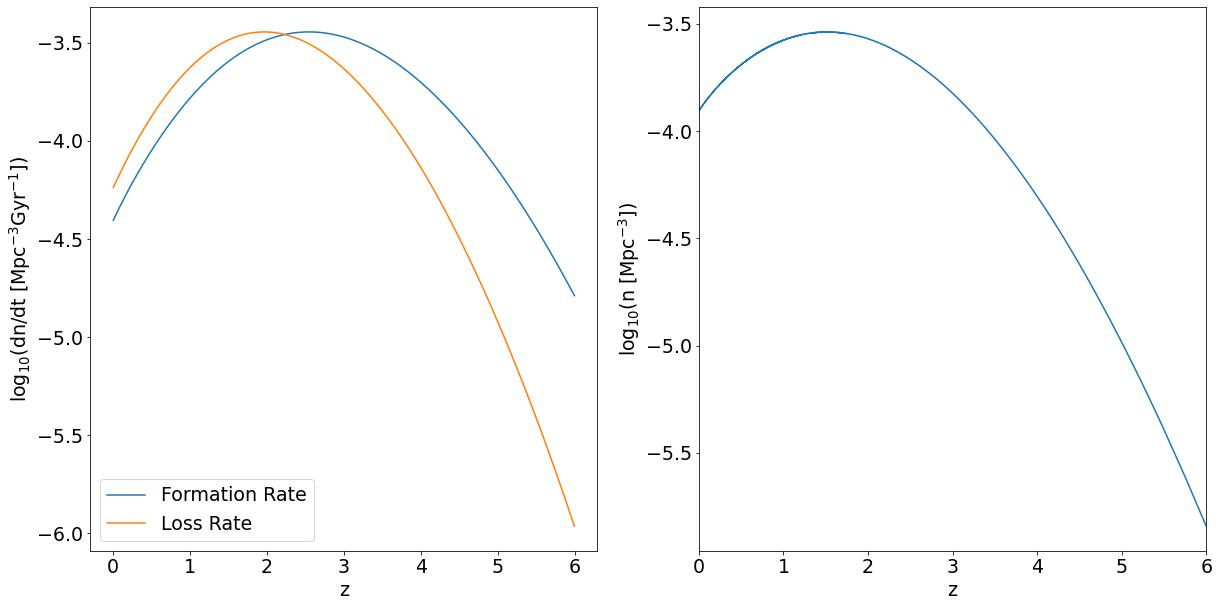
\includegraphics[width=\linewidth]{Plot_7_2.jpeg}
\caption{Left: Formation rate and loss rate of quasars as a function of redshift. The threshold halo mass for quasar formation is assumed here to have a constant value of $10^{12}M_\odot$. Right: Comoving number density of quasars as a function of redshift, calculated using Equation (8).}
\label{fig:7}
\end{figure}

\begin{figure}[H]
\centering
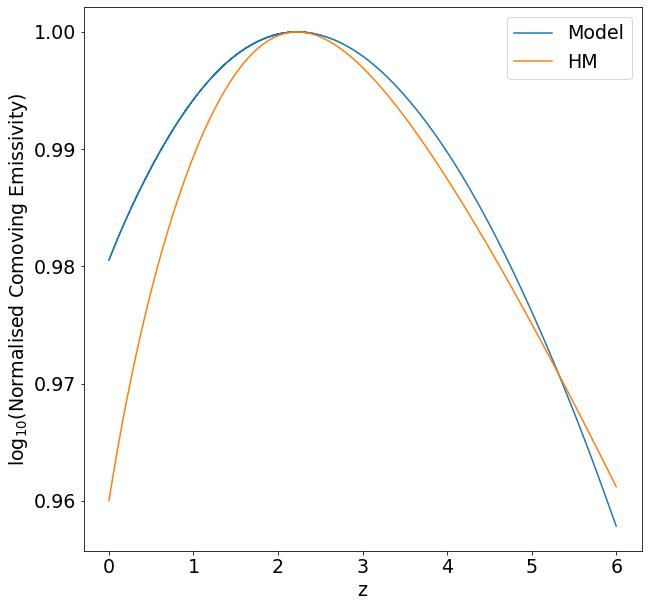
\includegraphics[width=12cm]{Plot_7_3.jpeg}
\caption{Comoving quasar emissivity as a function of redshift. The blue line shows the emissivity produced from our model using equation (10), and the orange line shows the emissivity at 912\AA \: calculated by \cite{Haardt_Madau} (Equation (11)). The emissivities peak at the same redshift and the model appears to be a good fit for the emissivity predicted by \citeauthor{Haardt_Madau} for $2\lesssim z\lesssim6$.}
\label{fig:8}
\end{figure}

\begin{figure}[H]
\centering
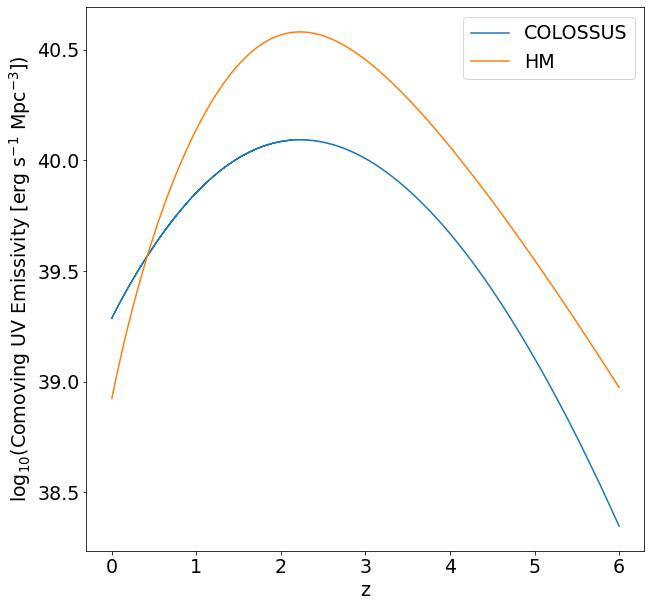
\includegraphics[width=12cm]{Plot_8.jpeg}
\caption{Comoving quasar UV emissivity as a function of redshift. The blue line shows emissivity calculated using Equation (16) and the orange line shows emissivity calculated from $\epsilon_{912}$ using Equation (14). The emissivity produced by our model is greater than $\varepsilon_{UV,HM}$ in this case.}
\label{fig:9}
\end{figure}

\twocolumngrid


For comparison, the emissivity calculated by our model must also be modified by introducing a factor $\eta_{UV}$ into Equation (9):

\begin{equation}
    E_{UV}=\eta_{UV}M_{BH,final}\eta c^2=\zeta\eta c^2
\end{equation}

\noindent where $\eta_{UV}$ is the fraction of energy released by the quasar in UV, and $\zeta=\eta_{UV}M_{BH}$ combines the two unknown quantities in this equation. Substituting this into Equation (10) gives our model's prediction for the quasar UV emissivity:

\begin{equation}
    \varepsilon_{UV,model}=n\frac{E_{UV}}{\tau}
\end{equation}

\noindent These emissivities are compared in Figure 9, where our model uses the values $M_{BH,final}=10^{8.5}M_\odot$ and $\eta_{UV}=0.5$. Our model's prediction for the emissivity is greater than $\varepsilon_{UV,HM}$ by $\sim1.0dex$ (1 order of magnitude). This difference could be due to the model's assumption that all halos which grow to masses higher than $10^{12}M_\odot$ will host quasars, which is obviously not true in reality, as the Milky Way and similar galaxies have halo masses $\geq10^{12}M_\odot$ and do not host quasars. Another potential reason for the difference is that the estimated values of $M_{BH,final}$ and $\eta_{UV}$ could be too large.\par

Currently, our model assumes that the critical mass above which halos will host quasars, $M_{H,crit}$, is constant, and that the quasar lifetime, $\tau$, is a significant fraction of the lifetime of the Universe, but these assumptions may not be true. In the next section, we introduce an alternative model for the case where quasar lifetimes are short and two alternative models which include a redshift-dependent $M_{H,crit}$.

\section{Introducing Alternative\\Models}

\subsection{Short Lifetime Case}

In the case where quasar lifetimes are small on the scale over which the formation rate varies, the comoving number density of quasars can be approximated as

\begin{equation}
    n\approx\frac{dn}{dt}\tau
\end{equation}

\noindent By substituting Equation (17) into Equation\\(16), obtain:

\begin{equation}
    \varepsilon_{UV,short}\approx\frac{dn}{dt}E_{UV}
\end{equation}

\noindent so the emissivity can be calculated without first obtaining the number density in this case, and is directly proportional to the quasar formation rate.\par

Comparing the plots in Figure 10 of quasar number density and UV emissivity produced using the short lifetime model with the initial model used in section 4 shows that the quasar UV emissivity produced by this model is closer to the initial model than either of the models described in section 5.2, this model also appears to produce a similarly good fit for $\varepsilon_{UV,HM}$ to the initial model. However, the quasar number density produced by this model is by far the lowest of any of the models shown in Figure 10. Quasars are assumed to release the same amount of energy during their lifetimes in all of these models, so short quasar lifetimes mean that the average luminosity of each quasar must be much greater. This cancels out the lower number density and leads to a similar magnitude for UV Emissivity to the initial model.

\subsection{Models with Variable Critical Mass}
\subsubsection{Keeping Virial Velocity Constant}

This model investigates the possibility that halos form quasars above a constant critical virial velocity, rather than a constant critical halo mass. The virial velocity of a halo is related to its mass by (\cite{Ikea}):

\begin{equation}
    v_H^2=\alpha(GM_H)^{\frac{2}{3}}(10H)^{\frac{2}{3}}
\end{equation}

\noindent where $\alpha=\frac{3}{5}$. Rearranging this and setting $v_H=v_{H,crit}=constant$ gives:

\begin{equation}
    M_{H,crit}(z)=\frac{v_{H,crit}^3}{10G\alpha^{\frac{3}{2}}}\frac{1}{H(z)}
\end{equation}

\noindent so $M{H,crit}$ decreases with redshift.\par

By comparing the plots from this model with the initial model in Figure 10, we see that this model produces significantly lower number densities of quasars and significantly lower UV emissivities than the initial model, with both being lower by $\sim1.0dex$. This is most likely because the constant virial velocity required to produce a good fit with $\varepsilon_{UV,HM}$ is $\sim300kms^{-1}$, which corresponds to a critical halo mass of $10^{13.3}M_\odot$ at $z=0$. This mass is significantly greater than the constant value used previously, and results in fewer halos crossing the mass threshold and forming quasars, which leads to the reduced magnitude of the emissivity. In section 6, the number densities of quasars will be compared with estimates by \cite{Hopkins}, and it will be shown that this model, as well as the short lifetime model in section 5.1, produce quasar number densities that are at least $1.0dex$ lower than the estimates of \citeauthor{Hopkins}

\onecolumngrid


\begin{figure}[H]
\centering
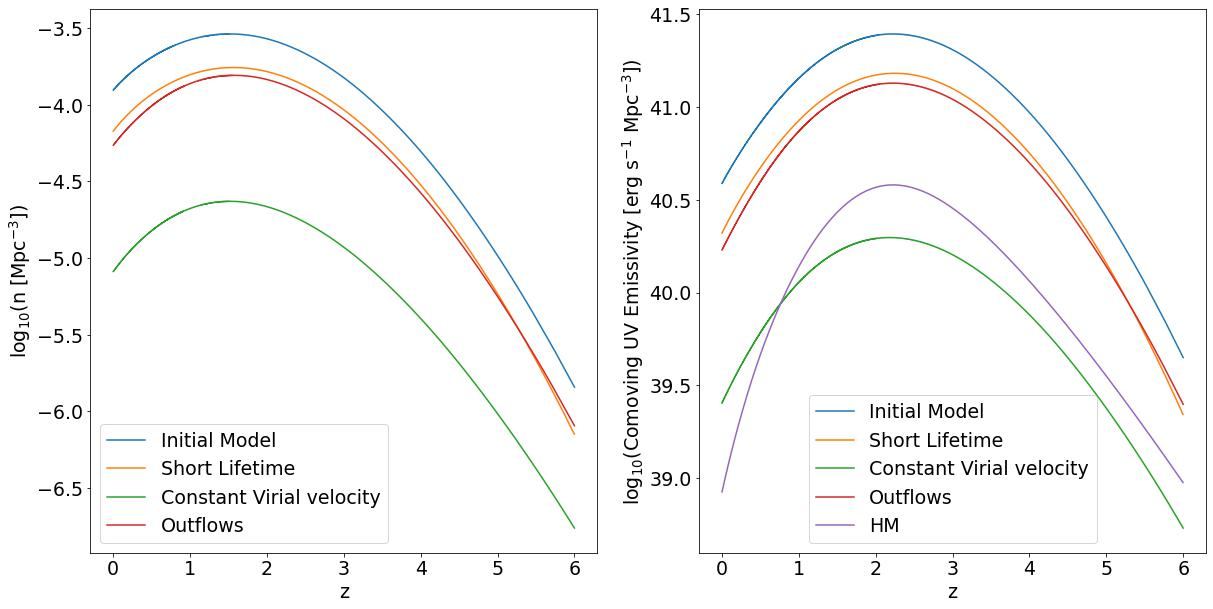
\includegraphics[width=\linewidth]{Plot_10.jpeg}
\caption{Left: Comoving number density of quasars plotted as a function of redshift. Produced using the initial model from section 4 (blue), the model with short quasar lifetimes (orange), the model where halos form quasars at a constant virial velocity (green), and the model where halos form quasars once star formation-driven outflows are no longer buoyant (red). All have been calculated using Equation (8), except for in the short lifetime model, which uses Equation (17). Right: Comoving quasar UV emissivity plotted as a function of redshift. Lines are coloured as on the left, where all have been calculated from the number densities on the left using Equation (16), except for in the short lifetime model, which uses Equation (18).The purple line shows the emissivity calculated from $\epsilon_{912}$ using Equation (14).}
\label{fig:10}
\end{figure}
\twocolumngrid


\subsubsection{Star Formation-Driven Outflows}

In \cite{Quasar}, the buoyancy of outflows of gas from the galaxy driven by star formation is found to be dependent on the mass of the host halo. By comparing the 'adiabat' of the outflow to that of the host galaxy's diffuse corona, the critical halo mass, above which outflows would no longer be buoyant, is

\begin{equation}
    M_{H,crit}=M_0\Delta_z^{-\frac{3}{8}}
\end{equation}

\noindent where $M_0\sim10^{12}M_\odot$, and

\begin{equation}
    \Delta_z\equiv(\Omega_m(1+z)^3+\Omega_\Lambda)^{\frac{1}{3}}
\end{equation}

\noindent Above this critical halo mass, the outflows are trapped by the corona. Gas then builds up in the central regions of the galaxy, allowing the SMBH to begin growing rapidly. As in the previous case, this leads to a critical halo mass which decreases with redshift.\par

Comparison of the plots in Figure 10 shows that, for $M_0=10^{12.4}M_\odot$, this model produces a similarly good fit for the evolution of $\varepsilon_{UV,HM}$ between redshifts 2 and 6 to the initial model, and produces quasar number densities and UV emissivities which are much closer to the constant $M_{H,crit}$ case than the model where virial velocity is kept constant. Additionally, this model produces very similar quasar number densities and emissivities to the short quasar lifetime model described in section 5.1.

 The results shown so far have been produced using assumed values for $M_{H,crit}$, $M_{BH,final}$, $\eta_{UV}$, and $k$ (the proportionality constant in Equation (7)) which are simple estimates. In the next section, we will investigate the effect of varying the values of $M_{H,crit}$ and $k$ on the resulting emissivity, and determine values for $\zeta=\eta_{UV}M_{BH,final}$ which produce a good fit for the magnitude of the emissivity calculated from $\epsilon_{912}$.

\section{Investigating the Effects of Changing Parameters}
\subsection{Varying k and M$_{\mathrm{H,crit}}$}

In Figure 11, we investigate the effect of varying $M_{H,crit}$ and $k$ on the resulting emissivity, where larger values of $k$ correspond to longer quasar lifetimes and vice versa. On the left hand side, it can be seen that increasing $M_{H,crit}$ results in lower UV emissivity, as a higher critical halo mass means fewer halos will cross the mass threshold, so fewer halos will host quasars. The peak emissivity is also shifted to lower redshift for larger values of $M_{H,crit}$. On the right hand side, increasing the value of $k$ can be seen to have a similar effect to increasing $M_{H,crit}$, decreasing the emissivity and shifting the peak to lower redshift. This is believed to be because, in our model, the total energy emitted by each quasar during its lifetime is always assumed to be the same, so the increasing lifetimes of quasars leads to their average luminosity being lower. This has the effect of decreasing the quasar emissivity, which cancels out the increase to emissivity due to the number density of quasars being greater for longer quasar lifetimes. It can also be seen that, for small $(<0.1)$ $k$, the effect of changing $k$ on the resulting emissivity is very small. This is because for small $k$, the quasar lifetimes are small on the timescale over which the quasar formation rate varies, so the emissivity can be described by the short lifetime

\onecolumngrid


 \begin{figure}[H]
     \centering
     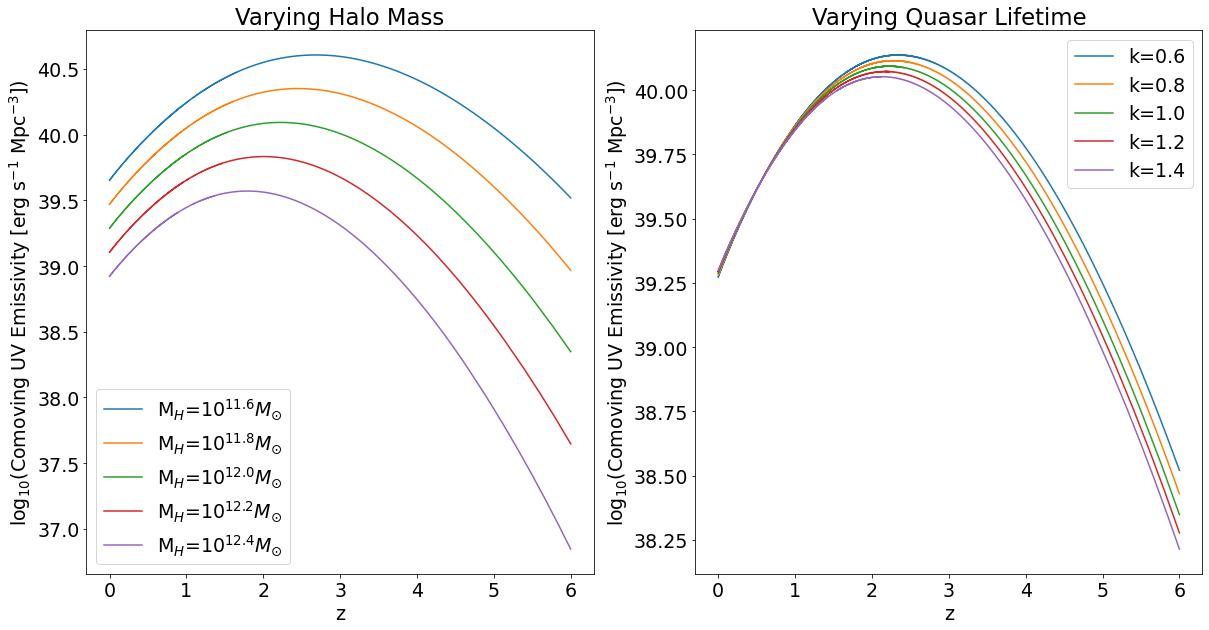
\includegraphics[width=\linewidth]{Plot_9.jpeg}
     \caption{Left: Comoving quasar UV emissivity plotted as a function of redshift, using the initial model described in section 4, for different values of $M_{H,crit}$. Greater values of $M_{H,crit}$ result in emissivities which peak at lower redshifts and have smaller magnitudes. Right: Comoving quasar UV emissivity plotted as a function of redshift, as on the left, for different values of the proportionality constant, $k$, in Equation (7). As for $M_{H,crit}$, Greater values of $k$ result in emissivities which peak at lower redshifts and have smaller magnitudes, but for small $k$, the effect of changing $k$ on the resulting emissivity is negligible.}
     \label{fig:11}
 \end{figure}

\begin{figure}[H]
\centering
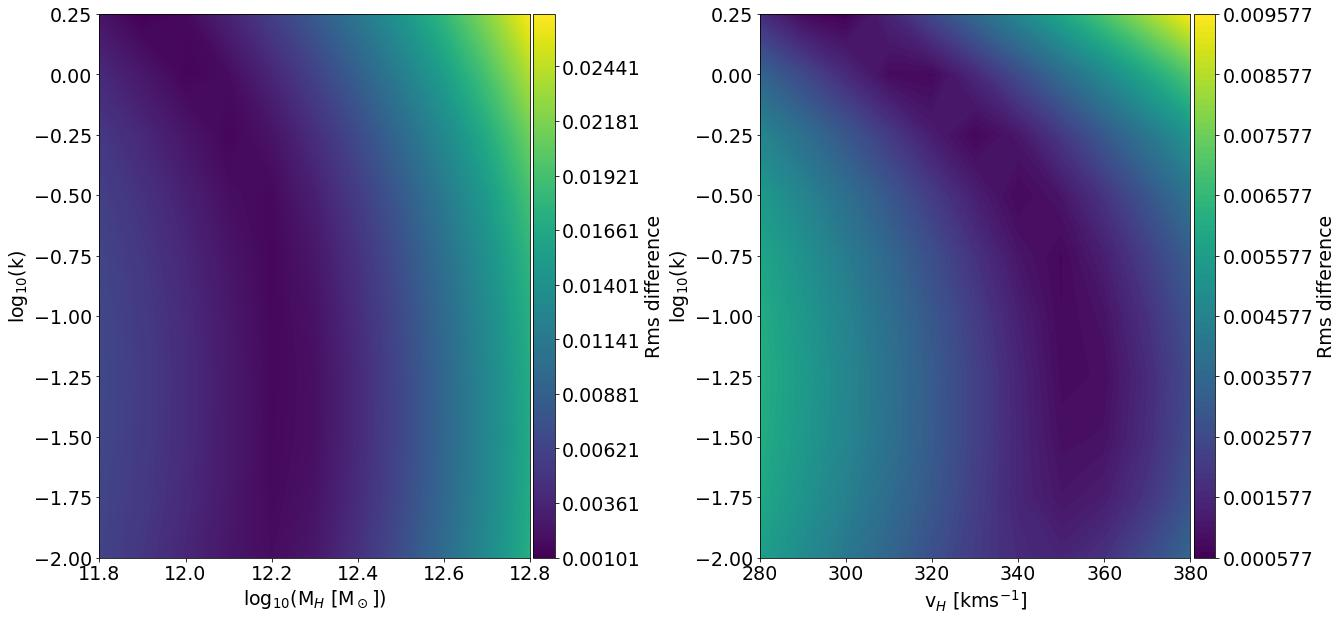
\includegraphics[width=9.5cm]{Plot_11.jpeg}
\caption{Top: Contour plot showing the variation of rms difference between the normalised curves of $\varepsilon_{UV,model}$ and $\varepsilon_{UV,HM}$ for different values of $M_{H,crit}$ and $k$ for the initial model in the redshift interval $2\leq z\leq6$. Middle: As above, but for the model where halos form quasars at a constant virial velocity. As such, the critical virial velocity, $v_{H,crit}$, replaces $M_{H,crit}$ on the x-axis. Bottom: As above, but for the model where halos form quasars once star formation-driven outflows are no longer buoyant. The critical halo mass at $z=0$, $M_0$, replaces $M_{H,crit}$ on the x-axis.}
\label{fig:12}
\end{figure}
\clearpage
\twocolumngrid


\noindent approximation discussed in section 5.1, and is directly proportional to the quasar formation rate as a result, as seen in Equation (18).\par

At this point, it is useful to provide a more quantitative description of how our model's fit with $\varepsilon_{UV,HM}$ varies as $M_{H,crit}$ and $k$ are chang\-ed. Figure 12 shows contour plots for the initial model, constant virial velocity model, and star formation-driven outflow model which describe how the model's fit for the evolution of $\varepsilon_{UV,HM}$ (or equivalently $\epsilon_{912}$) varies for different values of $M_{H,crit}$ and $k$ for $2\leq z\leq6$. The colour at each point represents the root mean square (rms) difference between the data points on the normalised curves for $\varepsilon_{UV,model}$ and $\varepsilon_{UV,HM}$ (such as the curves plotted in Figure 8). The short quasar lifetime model cannot be shown on a contour plot of this type, as the quasar emissivity produced by this model is independent of $k$.\par

It can be seen in Figure 12 that a low rms difference can be achieved for a large range of values of $M_{H,crit}$/$v_{H,crit}$/$M_0$ and $k$. For $k\lesssim0.3$, there is little variation in the rms difference for varying $k$. This is the same as in Figure 11, where the emissivity becomes significantly less dependent on $k$ for $k\lesssim0.1$. Apart from in the constant virial velocity model, the dependence on quasar lifetime also disappears for $k\gtrsim5.6$. This is most likely because, for high values of $k$, the quasar lifetime is several times greater than the dynamical timescale, $t_{dyn}$, and is equal to a large fraction of the age of the Universe, so the quasar loss rate lags behind the quasar formation rate to such an extent that quasar losses only become significant at low redshifts. This means that the majority of quasars that form at high redshifts will remain until after $z=2$, so the emissivity between redshifts 2 and 6 is no longer dependent on quasar lifetime. For $0.3\lesssim k\lesssim5.6$, our model's fit with $\varepsilon_{UV,HM}$ varies depending on both $M_{H,crit}$ and $k$, and it can be seen that if one of these quantities is increased, then the other must be decreased in order to maintain a low rms difference. This is also seen in Figure 11, where decreasing $k$ will have the opposite effect of increasing $M_{H,crit}$, and vice versa.\par

In summary, Figure 12 shows that there is a wide range of values for $k$ and $M_{H,crit}$/$v_{H,crit}$/$M_0$ for which the evolution of $\varepsilon_{UV,model}$ will be a good fit for the evolution of $\varepsilon_{UV,HM}$. To narrow down our model's estimates for the values of these quantities, we will need to introduce further criteria that must be satisfied for the selected values of $k$ and $M_{H,crit}$ to be considered viable.

\subsection{Using Black Hole Mass to Constrain k and M$_{\mathrm{H,crit}}$}

Since our model assumes that all halos that become quasar candidates will contain quasars, the UV emissivity produced should be greater than or similar to the true quasar UV emissivity. For each set of values of $k$ and $M_{H,crit}$, there will be a minimum required value of $\zeta=\eta_{UV}M_{BH,final}$ (Equation (15)) for which the peak value of $\varepsilon_{UV,model}$ will be equal to the peak value of $\varepsilon_{UV,HM}$:

\begin{equation}
    \zeta_{min}=\frac{\varepsilon_{HM,max}\tau_{max}}{\eta c^2n_{max}}
\end{equation}

\noindent where $\varepsilon_{HM,max}$ is the peak value of $\varepsilon_{UV.HM}$, and $\tau_{max}$ and $n_{max}$ are the values of $\tau(z)$ and $n(z)$ when $\varepsilon_{UV,model}$ is at its peak. If the required value of $\zeta$ is too low, then quasars do not become as massive as real quasars by the end of their lifetimes, and if the required value of $\zeta$ is too high, then quasars become significantly more massive than real quasars. It can be seen in Figure 4 of \cite{BH_mass_fns} that black hole mass functions (BHMFs) for type 1 quasars (quasars which are not obscured

\newpage

\onecolumngrid


\begin{figure}[H]
\centering
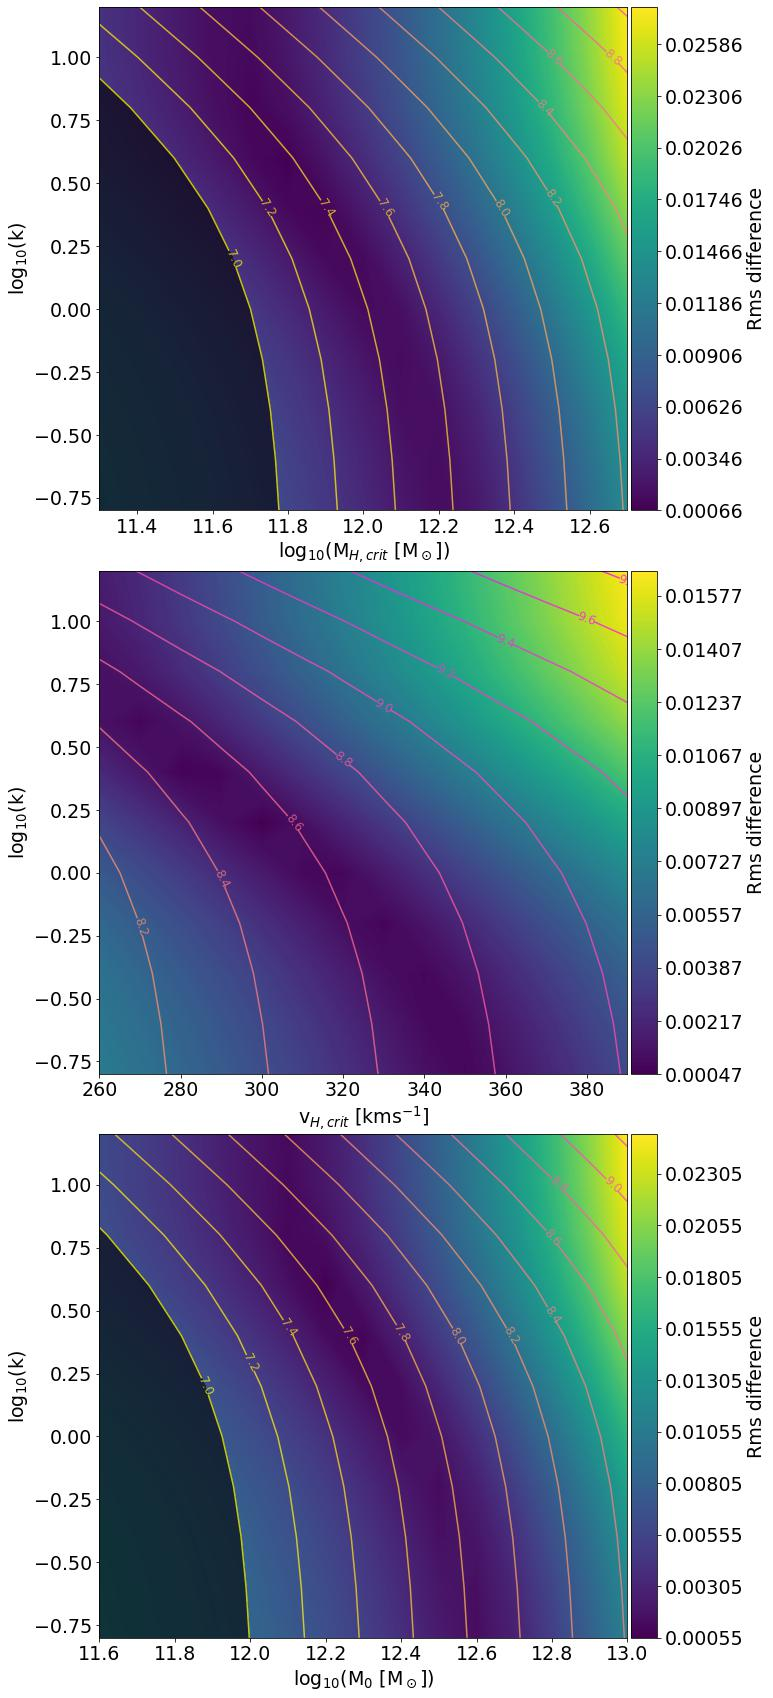
\includegraphics[width=10.25cm]{Plot_11_2.jpeg}
\caption{Underlying filled contour plots are the same as in Figure 12. The line contours show the required value of $log_{10}(\zeta_{min})$ to make $\varepsilon_{UV,model}$ equal to $\varepsilon_{UV,HM}$. The shaded areas mark where $\zeta_{min}$ must be below $10^7M_\odot$.}
\label{fig:13}
\end{figure}
\clearpage
\twocolumngrid


\noindent by dust) evolve with redshift, having a peak at $M_{BH}\sim10^{8.3}M_\odot$ with a maximum black hole mass of $\sim10^{10.5}M_\odot$ for $z=0.4$, and a peak at $M_{BH}\sim10^{9.7}M_\odot$ with black hole masses ranging between $\sim10^{8.5}-10^{11}M_\odot$ for $z=4.75$. The value of $M_{BH,final}=10^{8.5}M_\odot$ assumed in our model so far must therefore be an underestimate for redshifts higher than $z\sim0.5$.\par

The required values of $log_{10}(\zeta_{min})$ for different values of $k$ and $M_{H,crit}$ are shown as line contours in Figure 13. The shaded areas show where the required value of $\zeta_{min}$ becomes too low, and quasars do not have high enough black hole mass. In the areas of the initial model and star formation-driven outflow model plots (top and bottom plots respectively), where the rms difference is lowest, the minimum required val\-ue of $\zeta$ is $\sim2.0dex$ lower than the black hole mass where the BHMFs from \citeauthor{BH_mass_fns} peak, and in the areas of the constant virial velocity model plot (middle plot) where the rms difference is lowest, the minimum required val\-ue of $\zeta$ is $\sim1.0dex$ lower. The unknown factor of $\eta_{UV}$ in $\zeta$, which must be $<1$, could account for some of this difference, as $\eta_{UV}=0.1$ implies that the minimum value of $M_{BH,final}$ should be $\frac{\zeta_{min}}{0.1}$. Unless $\eta_{UV}\leq0.01$ (only a very small fraction of radiation from quasars is emitted in UV), this implies that the values of $\zeta$ should be significantly greater than $\zeta_{min}$ for the final masses of quasars to be accurate. For example, in the initial model, $\zeta_{min}$ must be approximately $10^{7.4-7.6}M_\odot$ for a low rms difference, but $M_{BH,final}$ should be $\sim2.0dex$ greater than this for the quasar black hole mass\-es to be accurate. This means that the peak emissivity produced by our model will be $\sim1-2\:dex$ greater than the peak value of $\varepsilon_{UV,HM}$, depending on $\eta_{UV}$.\par

The values of $\zeta_{min}$ for which the rms difference between $\varepsilon_{UV,model}$ and $\varepsilon_{UV,HM}$ is lowest are significantly higher ($\sim1.0dex$) in the model with constant virial velocity than in the other models. It can be seen in Figure 10 that, for a given value of $\zeta$, the constant virial velocity model produces by far the lowest emissivity, so a greater value of $\zeta_{min}$ is needed to make the peak emissivity equal to that of $\varepsilon_{UV,HM}$. On the other hand, $\zeta{min}$ only needs to be slig\-htly higher ($\sim0.2dex$) in the outflow model than in the initial model. Figure 10 also shows that, for a given $\zeta$, the emissivity produced by the outflow model is only slightly lower than for the initial model.\par

Introducing black hole mass as a constraint has provided us with estimates for the minimum required quasar black hole mass for each of our models, but has not narrowed down the values of $k$ and $M_{H,crit}$ any further than the original contour plot in Figure 12. This means that another parameter must be included as a constraint.

\subsection{Using Quasar Number Density to Further Constrain k and M$_{\mathrm{H,crit}}$}

As mentioned above, our model assumes that all quasar candidates will contain quasars, so the quasar number density predicted by our model should be greater than or similar to the true quasar number density. Figure 9 in \cite{Hopkins} shows the number density of quasars predicted from the bolometric quasar luminosity function (QLF). Since the number densities are split into groups with different luminosities, the peak number density in the bolometric case (top left in Figure 9 of \citeauthor{Hopkins}) is taken to be at $z\approx1$, where the luminosity interval with the highest number density is at its peak. Summing the number densities over all of the luminosity intervals for the bolometric number density at $z=1$ gives a peak observed quasar number density of $n_{obs}=10^{-3.45}Mpc^{-3}$.

\onecolumngrid


\begin{figure}[H]
\centering
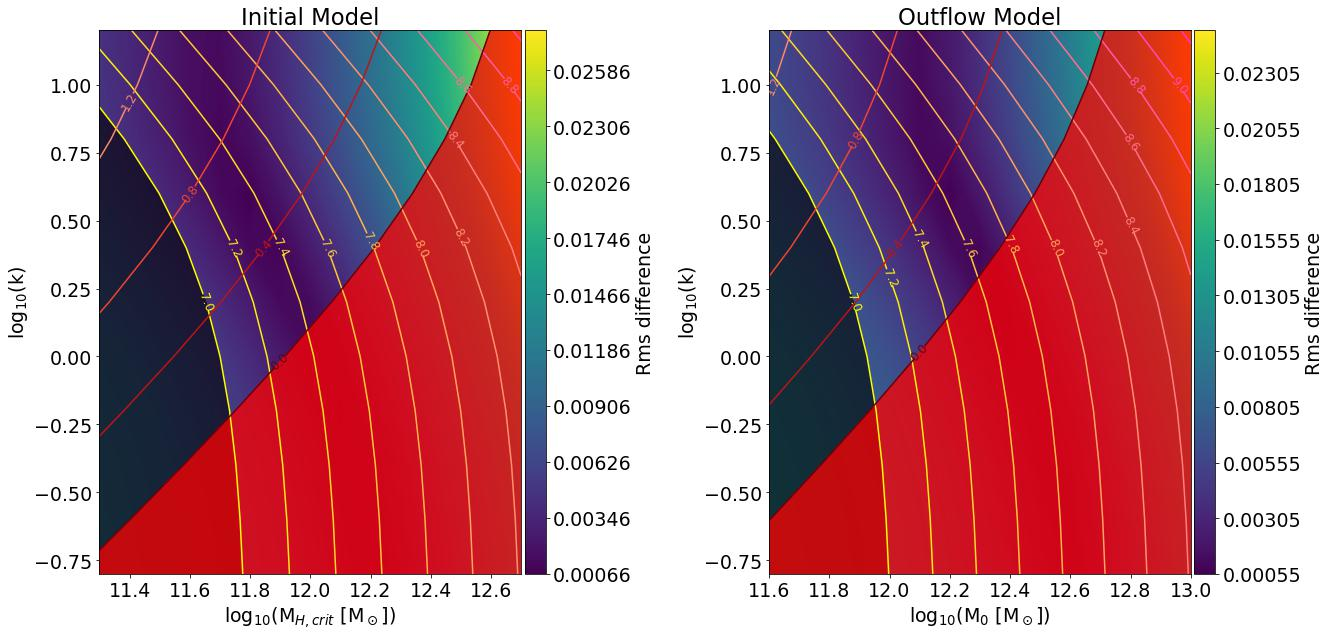
\includegraphics[width=\linewidth]{Plot_11_4.jpeg}
\caption{Underlying filled contour plots are the same as in Figure 12. The line contours and shaded areas from Figure 13 are also shown. The new line contours show the value of $log_{10}(\chi)$, and the red shaded areas show where $\chi<1$. The left plot shows the initial model, and the right plot shows the star formation-driven outflow model.}
\label{fig:14}
\end{figure}

\twocolumngrid


The quantity $\chi$ is equal to $\frac{n_{model}}{n_{obs}}$, where $n_{model}$ is the peak quasar number density in our model. The variation of $log_{10}(\chi)$ for different values of $k$ and $M_{H,crit}$ (left) or $M_0$ (right) is shown in Figure 14 as line contours, which are approximately perpendicular to the previous contours shown in Figure 13 and change from red to white with increasing $\chi$. The red shaded areas mark where $\chi<1$, i.e. where our model's prediction of quasar number density is lower than $n_{obs}$. The values of $k$ and $M_{H,crit}$ in these areas are not considered viable as, in these cases, our model predicts that there will be fewer quasar candidates than there are quasars in the real Universe. The model with constant virial velocity is omitted from Figure 14 as $\chi<1$ for all values of $k$ and $v_{H,crit}$ that result in a good fit with $\varepsilon_{UV,HM}$. The same is true for the short lifetime model, which produces significantly lower ($\sim2.0dex$) peak number densities than $n_{obs}$. As a result of this, the constant virial velocity model and short lifetime model cannot be considered viable under this constraint. For both of the remaining models (the initial model and the star formation-driven outflow model), the constraint that $\chi$ must be $>1$ restricts our model to using low ($\lesssim10^{12.1}M_\odot$ for the initial model and $\lesssim10^{12.3}M_\odot$ for the outflow model) values of $M_{H,crit}$/$M_0$, as well as high ($\gtrsim1.0$ for the initial model and $\gtrsim1.5$ for the outflow model) values of $k$ in order to maintain a low rms difference with $\varepsilon_{UV,HM}$. However, the allowed area still contains a large range of values of $k$ and $M_{H,crit}$/$M_0$.\par

From calculating the required values of $\zeta_{min}$ in the previous section, we know that for both of the remaining models, the value of $\zeta=\eta_{UV}\times M_{BH,final}$ required for the peak value of $\varepsilon_{UV,model}$ to be equal to the peak value of $\varepsilon_{UV,HM}$ is $\sim2.0\:dex$ lower than the masses of quasars at $2\leq z\leq6$. Therefore, if we assume that the unknown quantity $\eta_{UV}$ cannot account for all of this difference, then the true value of $\zeta$ must be $\gg\zeta_{min}$, and as a result of this, $\varepsilon_{UV,model}\gg\varepsilon_{UV,HM}$. In other words, the emissivity produced by our model must be an overestimate for the true quasar UV emissivity. The only way that this can be true is if the quasar number density assumed by our model is much gre-\\ater than the true number density of quasars, i.e. if $\chi\gg1$. In Figure 14, this corresponds to the highest ($\gtrsim10^{0.75}$) values of $k$, where the loss rate of quasars is negligible for $z<2$ as discussed in section 6.1. For these values of $k$, the evolution of the emissivity is independent of quasar lifetime for $2\leq z\leq6$, so $M_{H,crit}$ \& $M_0$ must be within the constant intervals $10^{11.65}\leq M_{H,crit}\leq10^{11.80}M_\odot$ and $10^{12.00}\leq M_0\leq10^{12.15}M_\odot$ for a low rms difference.

\subsection{Our Model with Optimised Parameters}

In this section, we present an example of what our model would look like with values of $k$, $M_{H,crit}$, $M_0$, and $\zeta$ that satisfy the requirements set by the constraints applied in sections 6.2 and 6.3. The emissivities produced by our initial model with an optimised value of $M_{H,crit}=10^{11.73}M_\odot$ \& our outflow model with $M_0=10^{12.08}M_\odot$ are shown in Figure 15. In both cases, we use $k=10$ and $\zeta=0.5\times10^{9.5}=10^{9.2}M_\odot$. Comparing Figure 8 with the left plot of Figure 15, the emissivities from our models now appear to peak at lower redshifts, but appear to fit the evolution of $\epsilon_{912}$ more closely for $2\leq z\leq6$ than in Figure 8 for both the initial and outflow models. Comparing Figure 9 with the right plot of Figure 15, we find that the difference in magnitude bteween $\varepsilon_{UV,model}$ and $\varepsilon_{UV,HM}$ is $\sim1.5dex$ in Figure 15 for both the initial and outflow models, which is greater than in Figure 9. However, as explained earlier in this section, $\varepsilon_{UV,model}$ is expected to be greater than $\varepsilon_{UV,HM}$ by $\sim1-2\:dex$, so this difference is

\onecolumngrid


\begin{figure}[H]
\centering
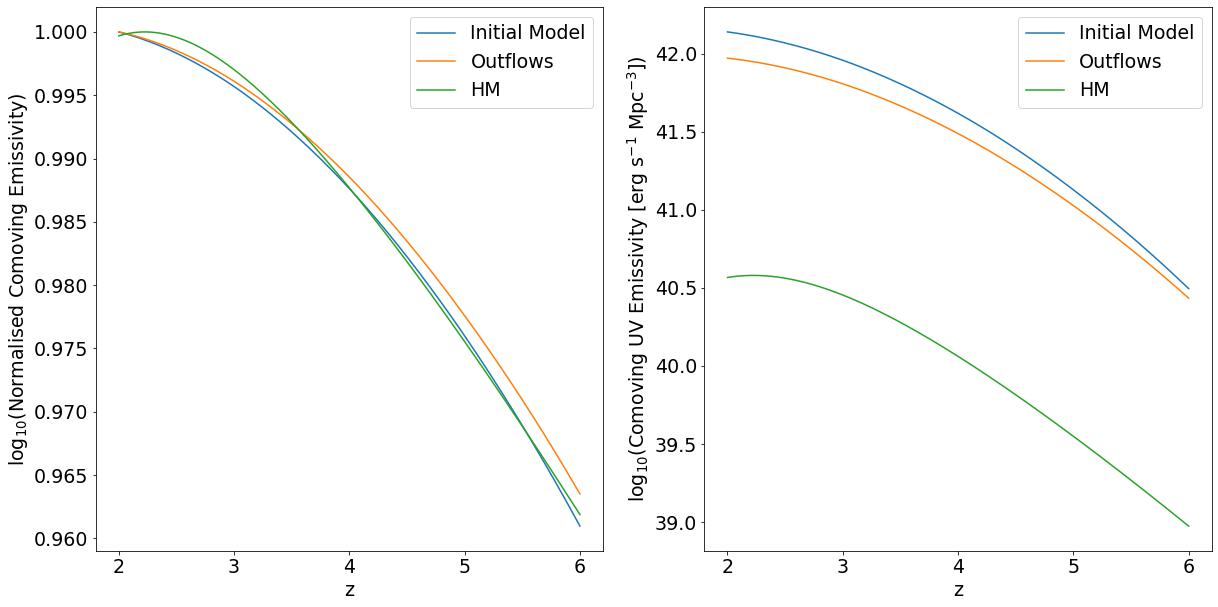
\includegraphics[width=\linewidth]{Plot_14.jpeg}
\caption{Left: Comparison of the normalised comoving quasar emissivities produced by our initial model (blue), our star formation-driven outflow model (orange), and $\epsilon_{912}$ (green), plotted as a function of redshift for $2\leq z\leq6$, using $M_{H,crit}=10^{11.73}M_\odot$ \& $k=10$ for the initial model, and $M_0=10^{12.08}M_\odot$ \& $k=10$ for the outflow model. Apart from the peak of $\epsilon_{912}$ being at lower redshift, both models appear to fit the evolution of $\epsilon_{912}$ well. Right: Comparison of the comoving quasar UV emissivities produced by our initial model (blue), our star formation-driven outflow model (orange), and $\varepsilon_{UV,HM}$ (green), plotted as a function of redshift for $2\leq z\leq6$. The emissivity from both of our models is $\approx1.5dex$ greater than $\varepsilon_{UV,HM}$. Both plots use $\zeta=0.5\times10^{9.5}=10^{9.2}M_\odot$.}
\label{fig:15}
\end{figure}

\twocolumngrid


\noindent within acceptable limits, and is assumed to be due to the quasar number density predicted by our model being greater than the true quasar number density. We can see from Figure 12 that the value of $k=10$ used to produce Figure 15 is above the minimum value of $k$ where the dependence on quasar lifetime vanishes due to the loss rate being negligible for $2\leq z\leq6$. Since the only acceptable values of $k$ are significantly greater than 1, this could provide evidence that our original assumption that quasar lifetimes are related to the dynamical timescale of their host halos is false, and that quasar lifetimes are instead long enough that the loss rate of quasars only becomes significant after $z=2$.

It is widely accepted that AGN feedback occurs in galaxies with halo mass \hspace{1mm} $M_H\gtrsim10^{12}\\M_\odot$ (\cite{Ikea}, \cite{Byrne}, \cite{Bassini}, \cite{Somerville}), and so for the new intervals for acceptable values of $M_{H,crit}$ and $M_0$ inferred from Figure 14, the initial model has $M_{H,crit}$ below this value, whereas the outflow model has a minimum possible value for $M_0$ of $\approx10^{12}M_\odot$. Additionally, it can be seen in Figure 12 that the minimum rms difference between the normalised curves of $\varepsilon_{UV,model}$ and $\epsilon_{912}$ is lower for the outflow model than for the initial model (the minimum rms difference is actually lowest for the constant virial velocity model, but as discussed earlier in this section, this model cannot be considered due to the extremely low number densities of quasars it produces). This means that, for optimal values of $k$ and $M_0$, the outflow model results in a better fit for the evolution of $\epsilon_{912}$ than the initial model. While this evidence points towards the outflow model being the best out of all of our models, it does not provide a suitable reason to reject our initial model, and so under the constraint that the peak value of the quasar number density produced by our model must exceed $n_{obs}=10^{-3.45}Mpc^{-3}$, both the outflow model and the initial model can still be considered.

\section{Limitations and Further\\Work}

Although our model successfully reproduces the redshift evolution of comoving quasar UV emissivity, we have identified several issues\\which must be resolved in order to improve our model. In this section, we will discuss some of these limitations, and how they could be addressed in the future.\par

The first of these limitations is the way in which our model calculates the formation rate of quasars. Currently, our model assumes that every halo whose mass increases above $M_{H,crit}$ will then contain a quasar. As mentioned in section 4.2, this cannot be true as many Milky Way-like galaxies (including the Milky Way itself) have halo masses $\geq10^{12}M_\odot$. Using the final values of $M_{H,crit}$/$M_0$ from Figure 15, we find that many Milky Way-like galaxies will be assumed to host quasars according to our model. An obvious result of this problem is that the quasar number densities and hence the quasar emissivities predicted by our model will be greater than their true values. There are multiple ways in which this limitation could be improved. The simplest method would be to assume that only a fraction of quasar candidates will host quasars:

\begin{equation}
    n_{qso}=\phi n_{candidates}
\end{equation}

\noindent where $n_{qso}$ and $n_{candidates}$ are the comoving number densities of quasars and quasar candidates respectively, and $0<\phi\leq1$. The problem with this method is that it introduces another unknown quantity, $\phi$, into the calculation of quasar emissivity. Without knowing $\eta_{UV}$ it would be impossible to determine the value of $\phi$. Another possibility would be to investigate other factors which affect quasar evolution, such as quasar clustering (\cite{Clustering_1}, \cite{Clustering_2}) and the morphology of the host galaxy (\cite{Morphology}), and determine whether these can be used to further restrict which galaxies can host quasars. If successful, this method would neg\-ate the need to introduce a further unknown quantity into the calculation of quasar emissivity.\par

Another limitation is that our model does not consider the properties of individual quas\-ars, such as individual mass or instantaneous luminosity. Apart from quasar lifetime, which depends on redshift (Equation (7)), all quasars are considered to be the same. The quasars in our model have the same final mass, are always active, and are always at their time-averaged luminosity. A potential method to improve upon this limitation is to incorporate the duty cycles of quasars into our model. The duty cycle is the fraction of each quasar's lifetime for which it is active. Using this method would remove the current model's approximation that quasars are active throughout their\\whole lifetimes, and would most likely decre\-ase the difference between $\varepsilon_{UV,model}$ and\\$\varepsilon_{UV,HM}$. Another method would be to produce a distribution of final quasar masses using BHMFs such as the ones from \citeauthor{BH_mass_fns} discussed in section 6.2 instead of using a constant value for $M_{BH,final}$. To test the effectiveness of these methods, we could also attempt to produce a quasar luminosity function using our model and compare this with the predictions of \cite{Hopkins}. For simplicity, it may be necessary to assume that all quasars are at their Eddington luminosity.\par

Lastly, in order to make comparisons to $\epsilon_{912}$, we converted the bolometric quasar emissivity produced by our model into the UV emissivity using the factor $\eta_{UV}$. However, $\eta_{UV}$ is not known, and so we can only obtain estimates for the product of the two unknown quantities: $\zeta=\eta_{UV}M_{BH,final}$. This could be solved by comparing $\varepsilon_{model}$ to the true quasar emissivities in different regions of the EM spectrum. This would remove the need to use $\eta_{UV}$ and allow us to estimate $M_{BH,final}$ directly, instead of $\zeta$.

\section{Conclusions}

The aim of this project was to develop a model for the formation and evolution of quasars based on the relationship between the evolution of quasars and their host galaxies. Our model assumed that the formation rate of quasars was equal to the rate at which galactic halos cross a halo mass threshold, $M_{H,crit}$. The other main assumption made by our model was that the lifetimes of quasars are related to the dynamical timescale of their host halos. We also investigated alternative models, in which quasar lifetimes were assumed to be short on the time-\\scale over which the quasar formation rate varies, and where $M_{H,crit}$ varied with redshift, for either a constant critical halo virial velocity, $v_{H,crit}$, or for the halo mass above which star formation-driven outflows are no longer buoyant.\par

We used the quasar formation rate calcuated from our model to estimate the comoving number density, and subsequently the comoving UV emissivity, of quasars for $0\leq z\leq6$. Initial tests with constant $M_{H,crit}$ were compared with the comoving quasar emissivity at 912\AA, $\epsilon_{912}$, calculated by \cite{Haardt_Madau}. This revealed that our model's estimate for quasar UV emissivity was a good fit for the redshift evolution of $\epsilon_{912}$. Tests of the other models resulted in similarly good fits for the evolution of $\epsilon_{912}$, but the magnitudes of quasar number density and emissivity varied over $\sim2.0dex$ for different models.\par

Comparing quasar number densities with those calculated by \cite{Hopkins} show\-ed that the constant virial velocity and short lifetime models could not be used, as they produced quasar number densities which were significantly lower than the predictions of \citeauthor{Hopkins} By estimating the minimum black hole masses required for our model's estimates for UV emissivity to equal the UV emissivity calculated from $\epsilon_{912}$ and comparing to the quasar BHMFs calculated by \cite{BH_mass_fns}, we were able to conclude that both our initial model and our star formation-driven outflow model predict UV emissivities that are $\sim1-2\:dex$ greater than the UV emissivity calculated from \citeauthor{Haardt_Madau}, depending on the fraction of energy released by quasars in UV. This in turn means that our models should predict quasar number densities that are significantly greater than the values given in \citeauthor{Hopkins}\par

Using these constraints, we conclude that both the initial model and the outflow model were found to be viable, with optimal values of $M_{H,crit}=10^{11.73}M_\odot$ for the initial model and $M_0=10^{12.08}M_\odot$ for the outflow model. The optimum quasar lifetime was found to be $\sim10\times$ the dynamical timescale of the host halo, and the black hole mass of each quasar was assumed to be $M_{BH,final}=10^{9.5}M_\odot$. Using these parameters, both models were found to fit the evolution of $\epsilon_{912}$ well for $2\leq z\leq 6$.\par

With the current limitations of our model, it can only be used to predict the redshift evolution of quasar emissivity. As such, its usefulness as a tool to estimate the properties of quasars is limited. However, if the limitations of our model can be addressed with further work, then it may become possible to estimate other global properties of quasars using our model, such as their number density and the magnitude of their emissivity. It may also be possible to calculate quasar luminosity functions using the emissivity predicted by our model. If these improvements can be made, then our model will be a useful tool for estiating the properties of quasars, and hence their effect on the Universe.

\bibliographystyle{unsrtnat} % {mn2e}
\bibliography{citation.bib}

\end{document}